\documentclass[letterpaper,12pt]{article}
\usepackage[utf8]{inputenc}
\usepackage{graphicx}
\usepackage{amssymb,amsmath}
\usepackage{verbatim}
\usepackage[parfill]{parskip}
\usepackage{hyperref}
\usepackage{listings}

\title{Information Retrieval CS 834 : Assignment 4}
\author{Miranda Smith\\ msmit213@odu.edu}
\begin{document}
\maketitle
\date{}

\begin{abstract}
Exercise questions 8.3, 8.4 , and 8.5 completed. Spring 2017. 
\end{abstract}

\pagebreak

\section{Problem 8.3}
For one query in the CACM collection (provided at the book website), generate a ranking using Galago, and then calculate average precision, NDCG at 5 and 10, precision at 10, and the reciprocal rank by hand.

\subsection{Solution}

I chose query 27 from the CACM collection. 

\begin{lstlisting}[breaklines]
memory management aspects of operating systems
\end{lstlisting}

I created an index for the cacm.corpus with Galago. Then I ran Galago with a batch-query to get the top 10 relavent documents, outputed to 83queryoutput.txt, shown below. 

\begin{lstlisting}[breaklines]
---------------------------------------------------
27 Q0 CACM-2297 1 -34.31623459 galago
27 Q0 CACM-2406 2 -35.42752838 galago
27 Q0 CACM-2357 3 -35.45236969 galago
27 Q0 CACM-1725 4 -35.51766968 galago
27 Q0 CACM-1752 5 -35.52021027 galago
27 Q0 CACM-2902 6 -35.60168457 galago
27 Q0 CACM-2988 7 -35.76276016 galago
27 Q0 CACM-2669 8 -35.86756134 galago
27 Q0 CACM-2798 9 -35.87216949 galago
27 Q0 CACM-2319 10 -35.92541885 galago
---------------------------------------------------
\end{lstlisting}

The relevant documents were obtained from the book website. For question 27 there are 29 relevant documents listed in 83relavancejudgements.txt.

I ran Galago eval to get the system evaluated metrics so that I could verify my hand done calculations.
\begin{lstlisting}[breaklines]
---------------------------------------------------
galago.bat eval 83queryoutput.txt 83relavancejudgements.txt
num_ret          27 10
num_rel          27 29
num_rel_ret      27 6
map              27 0.1298
ndcg             27 0.3006
ndcg15           27 0.4594
R-prec           27 0.0000
bpref            27 0.0000
recip_rank       27 1.0000
P5               27 0.4000
P10              27 0.6000
P15              27 0.4000
P20              27 0.3000
P30              27 0.2000
P100             27 0.0600
P200             27 0.0300
P500             27 0.0120
P1000            27 0.0060
---------------------------------------------------
\end{lstlisting}

\begin{lstlisting}[breaklines]
---------------------------------------------------
Doc 	Relevant
1	1
2	0
3	0
4 	0
5	1
6	1
7 	1
8	1
9	1
10	0
---------------------------------------------------
\end{lstlisting}
\subsubsection{Average Precision}

Comparing the returned documents to the relevant documents I found that the number of documents returned was 10 and the number of relevant documents returned was 6. 

\begin{center}
\begin{tabular}{ |c|c|c| } 
 \hline
 Doc & Rel & Precision \\ 
\hline
 1 & 1 & 1\\ 
 2 & 0 & 0.5\\ 
 3 & 0 & 0.33\\ 
 4 & 0 & 0.25\\ 
 5 & 1 & 0.4\\ 
 6 & 1 & 0.5\\ 
 7 & 1 & 0.57\\ 
 8 & 1 & 0.625\\ 
 9 & 1 & .666\\ 
 10 & 0 & 0.6\\ 
 \hline
\end{tabular}
\end{center}

$$Average Precision = \frac{1 + 0.4 + 0.5 + 0.57 + 0.625 + 0.666 }{6} = 0.627 $$


\subsubsection{NDCG at 5}

The NDCG is the normalized discounted cumulative gain. It is calculated with 
$$NDCG_5=\frac{DCG_5}{IDCG_5}$$

I made the assumption that the score would be 0 for a non-relevant document and 1 for a relevant document.

$$DCG_5 = \Sigma_{i=1}^5\frac{rel_i}{log_2(i+1)}$$


\begin{center}
\begin{tabular}{ |c|c|c|c| } 
 \hline
 Doc & Rel & log2(i+1)	& rel i/ log2(i+1) \\ 
\hline
 1 & 1 & 1 & 1\\ 
 2 & 0 & 1.585 & 0\\ 
 3 & 0 & 2 & 0\\ 
 4 & 0 & 2.322 & 0\\ 
 5 & 1 & 2.585 & 0.386\\ 
 \hline
\end{tabular}
\end{center}

Discounted Cumulative Gain = 1+0+0+0+0.386 = 1.386 


Ideal Discounted Cumulative Gain = 1 +  0.631 + 0 + 0 + 0 = 1.631

$$NDCG_5 = \frac{ 1.386 }{ 1.631} = .850 $$


\subsubsection{NDCG at 10}

\begin{center}
\begin{tabular}{ |c|c|c|c| } 
 \hline
 Doc & Rel & log2(i+1)	& rel i / log2(i+1) \\ 
\hline
 1 & 1 & 1 & 1\\ 
 2 & 0 & 1.585 & 0\\ 
 3 & 0 & 2 & 0\\ 
 4 & 0 & 2.322 & 0\\ 
 5 & 1 & 2.585 & 0.386\\ 
 6& 1 & 2.807 & 0.356\\ 
 7 & 1 & 3 & 0.333\\ 
 8 & 1 & 3.170 & 0.315\\ 
 9 & 1 & 3.322 & 0.301\\ 
 10 & 0 & 3.459 & 0\\ 
 \hline
\end{tabular}
\end{center}

Discounted Cumulative Gain = 1+ 0 + 0 + 0 + 0.386 + 0.356 + 0.333 + 0.315 + 0.301 + 0 = 2.691

Reorder the documents to put all the relevant ones first to get the ideal discounted cumulative gain.

Ideal Discounted Cumulative Gain = 1 +  0.631 + 0.5 + 0.431 + 0.386 + 0.356 + 0 + 0 + 0 + 0 = 3.304

$$NDCG_5 = \frac{ 2.691 }{ 3.304} = .814 $$


\subsubsection{Precision at 10}

$$Precision at 10 = \frac{Rel Docs Retrieved}{Docs Retrieved} = \frac{6}{10} = 0.6 $$

\subsubsection{Reciprocal Rank}
Reciprocal Rank is the reciprocal of the rank at which the first relevant document is retrieved.

First document is relevant meaning Reciprocal Rank = 1.


\pagebreak

\section{Problem 8.4}
For two queries in the CACM collection, generate two uninterpolated recall-precision graphs, a table of interpolated precision values at standard recall levels, and the average interpolated recall-precision graph.

\subsection{Solution}

I chose query 1 and 2. I ran the queries through Galago Batch-Search to get 20 returned documents and calculated the recall and precision at each point to generate the following graphs.

\begin{figure}
  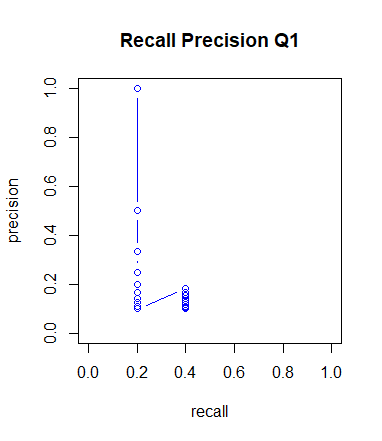
\includegraphics[width=\linewidth]{84q1uninterpolated.PNG}
  \label{fig:q1uninterpolated}
\end{figure}

\begin{figure}
  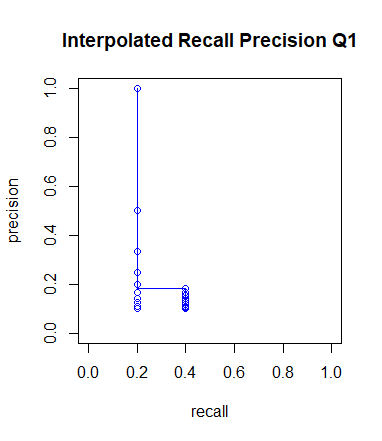
\includegraphics[width=\linewidth]{84q1interpolated.PNG}
  \label{fig:q1interpolated}
\end{figure}

\begin{figure}
  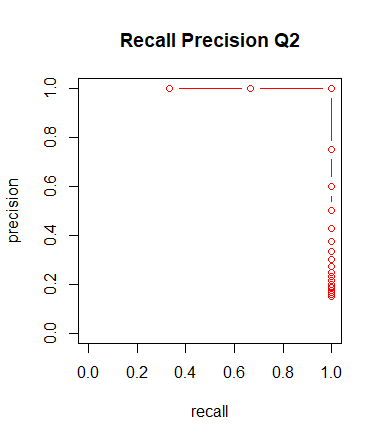
\includegraphics[width=\linewidth]{84q2uninterpolated.PNG}
  \label{fig:q2uninterpolated}
\end{figure}

\begin{figure}
  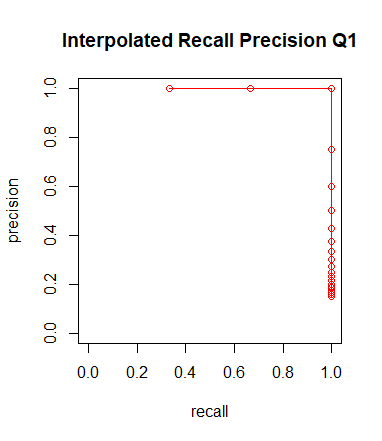
\includegraphics[width=\linewidth]{84q2interpolated.PNG}
  \label{fig:q2interpolated}
\end{figure}

\pagebreak

\begin{table}[h]
\centering
\begin{tabular}{ |c|c|c|c|c| } 
 \hline
 Doc & Rel & Recall & Precision & Interpolated Precision\\ 
\hline
1&1&0.2&1.&1. \\
2&0&0.2&.5&.5\\
3&0&0.2&.333&.333\\
4&0&0.2&.25&.25\\
5&0&0.2&.2&.2\\
6&0&0.2&.167&.182\\
7&0&0.2&.143&.182\\
8&0&0.2&.125&.182\\
9&0&0.2&.111&.182\\
10&0&0.2&.1&.182\\
11&1&0.4&.182&.182\\
12&0&0.4&.167&.167\\
13&0&0.4&.154&.154\\
14&0&0.4&.143&.143\\
15&0&0.4&.133&.133\\
16&0&0.4&.125&.125\\
17&0&0.4&.118&.118\\
18&0&0.4&.111&.111\\
19&0&0.4&.105&.105\\
20&0&0.4&.1&.1\\
 \hline
\end{tabular}
\caption{Question 1}
\end{table}

\begin{table}[h]
\centering
\begin{tabular}{ |c|c|c|c|c| } 
 \hline
 Doc & Rel & Recall & Precision & Interpolated Precision\\ 
\hline
1&1&.333&1.&1.\\
2&1&.667&1.&1.\\
3&1&1.&1.&1.\\
4&0&1.&.75&.75\\
5&0&1.&.6&.6\\
6&0&1.&.5&.5\\
7&0&1.&.429&.429\\
8&0&1.&.375&.375\\
9&0&1.&.333&.333\\
10&0&1.&.3&.3\\
11&0&1.&.273&.273\\
12&0&1.&.25&.25\\
13&0&1.&.231&.231\\
14&0&1.&.214&.214\\
15&0&1.&.2&.2\\
16&0&1.&.188&.188\\
17&0&1.&.176&.176\\
18&0&1.&.167&.167\\
19&0&1.&.158&.158\\
20&0&1.&.15&.15\\
 \hline
\end{tabular}
\caption{Question 2}
\end{table}

\pagebreak

\section{Problem 8.5}
Generate the mean average precision, recall-precision graph, average NDCG at 5 and 10, and precision at 10 for the entire CACM query set.

\subsection{Solution}

I ran the queries through galago's batch search. Then I used Galago eval to find the statistics for MAP, P@ 10, and NDCG at 10. Eval only gives NDCG at 15, however I limited the returned documents to 10 so the values should be equivalent. 

\begin{figure}
  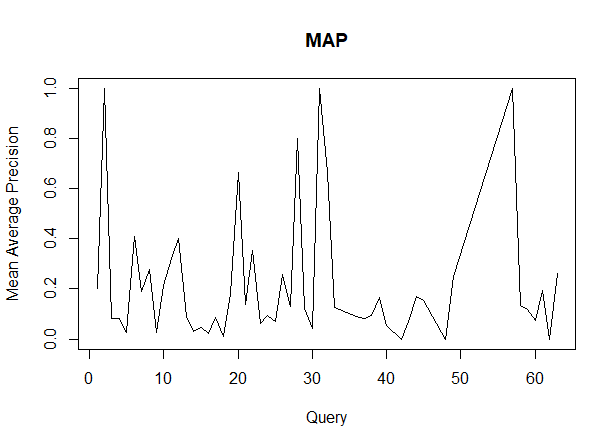
\includegraphics[width=\linewidth]{85map.PNG}
  \label{fig:CACM map}
\end{figure}

\begin{figure}
  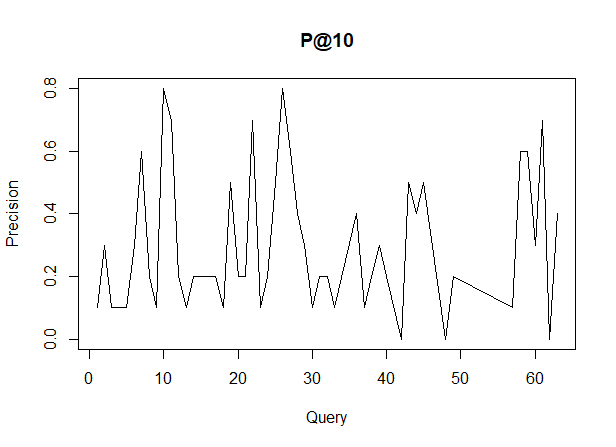
\includegraphics[width=\linewidth]{85p10.PNG}
  \label{fig:CACM p10}
\end{figure}

\begin{figure}
  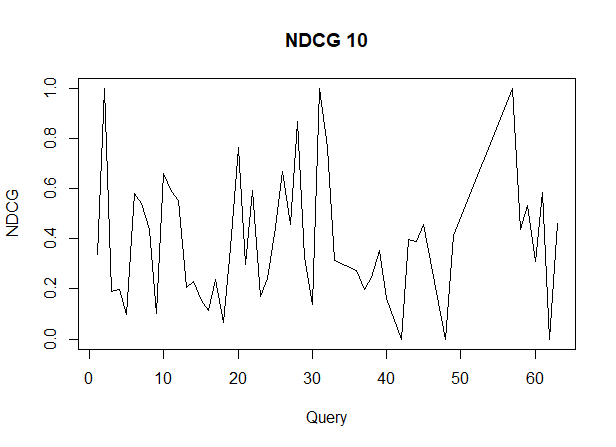
\includegraphics[width=\linewidth]{85ndcg10.PNG}
  \label{fig:CACM ndcg 10}
\end{figure}


\end{document}